\NewChapter{Up to Heaven}

\quote{看哪,他们都是一样的人,说着同一种语言,如今他们既然能做起这事,以后他们想要做的事就没有不成功的了。}{《创世记》}

三个凡人各自召集了一批士兵踏上弑神之旅,神位于“上帝之山”迦密山(Carmel)山顶的圣殿,想要达成目标必须确保三个凡人阵营都有任一士兵到达圣殿。在前进时神会对他们的道路地形进行干扰,三人只有利用自己的能力相互合作才能实现目标。

\section{创作背景}
游戏创作于2022年8月,为南加州大学游戏暑期工作坊设计的基于《Tabletop Simulator》桌游模拟器的桌面游戏。团队由四人组成,\textbf{最终荣获“Balanced Cooperative Characters Award”。}

\section{游戏简介}
《Up to Heaven》灵感源自经典桌游《Up the River》,是一款四人非对称对抗PVP游戏。三名玩家会扮演三个不同的人类角色合作登上天堂:骑士、皇帝、牧师。一名玩家扮演全知全能的上帝阻止玩家登上天堂。

每个人类角色有两枚棋子,若骑士、皇帝、牧师都至少有一枚棋子到达天堂则人类胜利。若某一角色的棋子全部淘汰或卡组中的牌已被抽完则上帝胜利。

\begin{figure}[H]
    \centering
    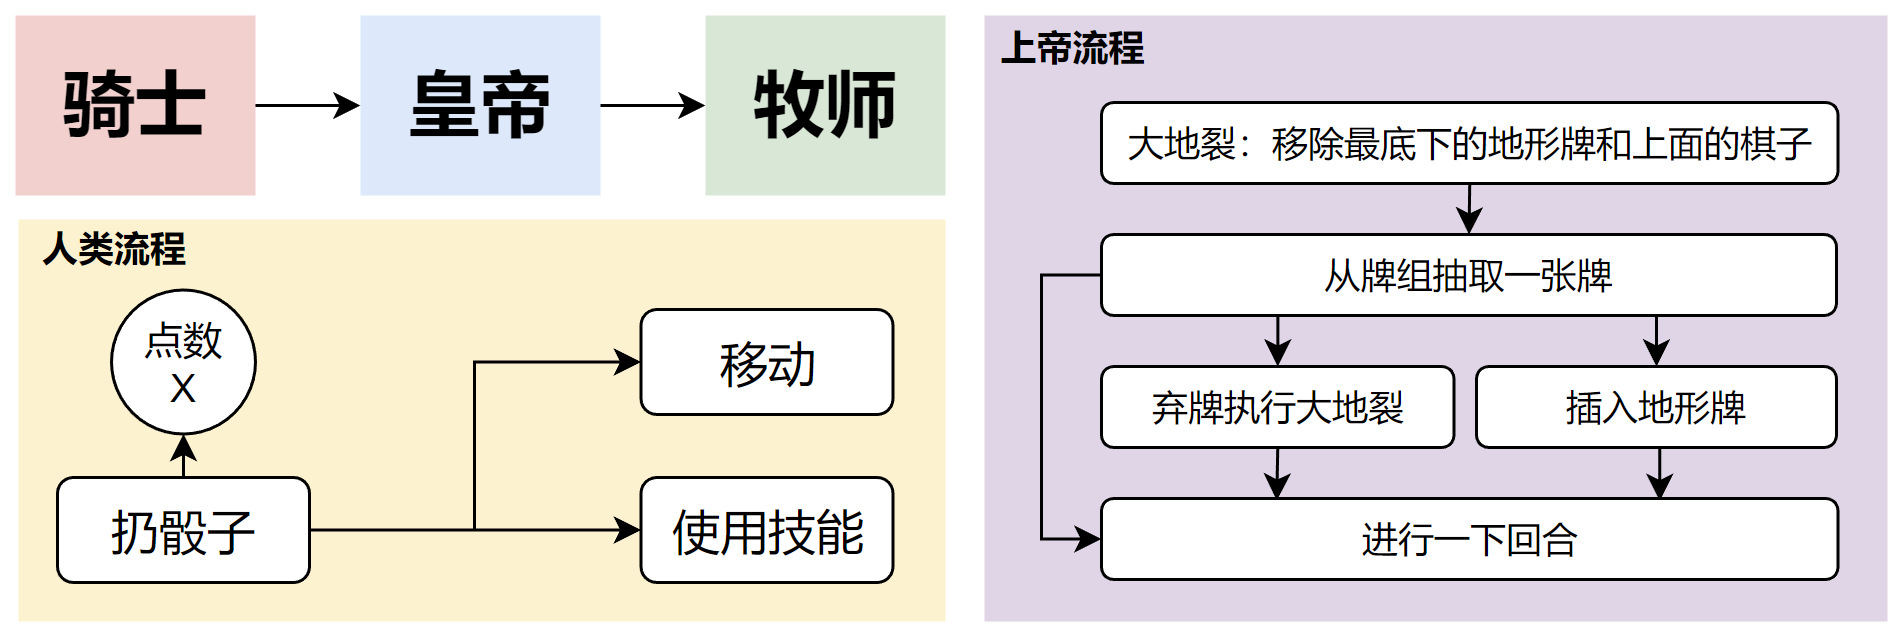
\includegraphics[width=0.9\textwidth]{Images/Up to Heaven/preocess.png}
    \caption{Up to Heaven\ 游戏简化流程}
    \label{fig:UTH_Process}
\end{figure}

\section{设计思路}
我们保留了原桌游《Up the River》每回合会从末端删除卡的设定,并把把原本的对称PVP游戏改为非对称PVP游戏。

我们将能力拆解到三个不同的人类,并以“角色机制和角色身份相符”的目标设计角色,以带给玩家足够的沉浸感和扮演感。而全知全能的上帝应该是强大,让人类感到恐惧的。上帝有改变地形的能力,且在游戏初期让玩家感觉的可怕和无奈。

\begin{figure}[H]
    \centering
    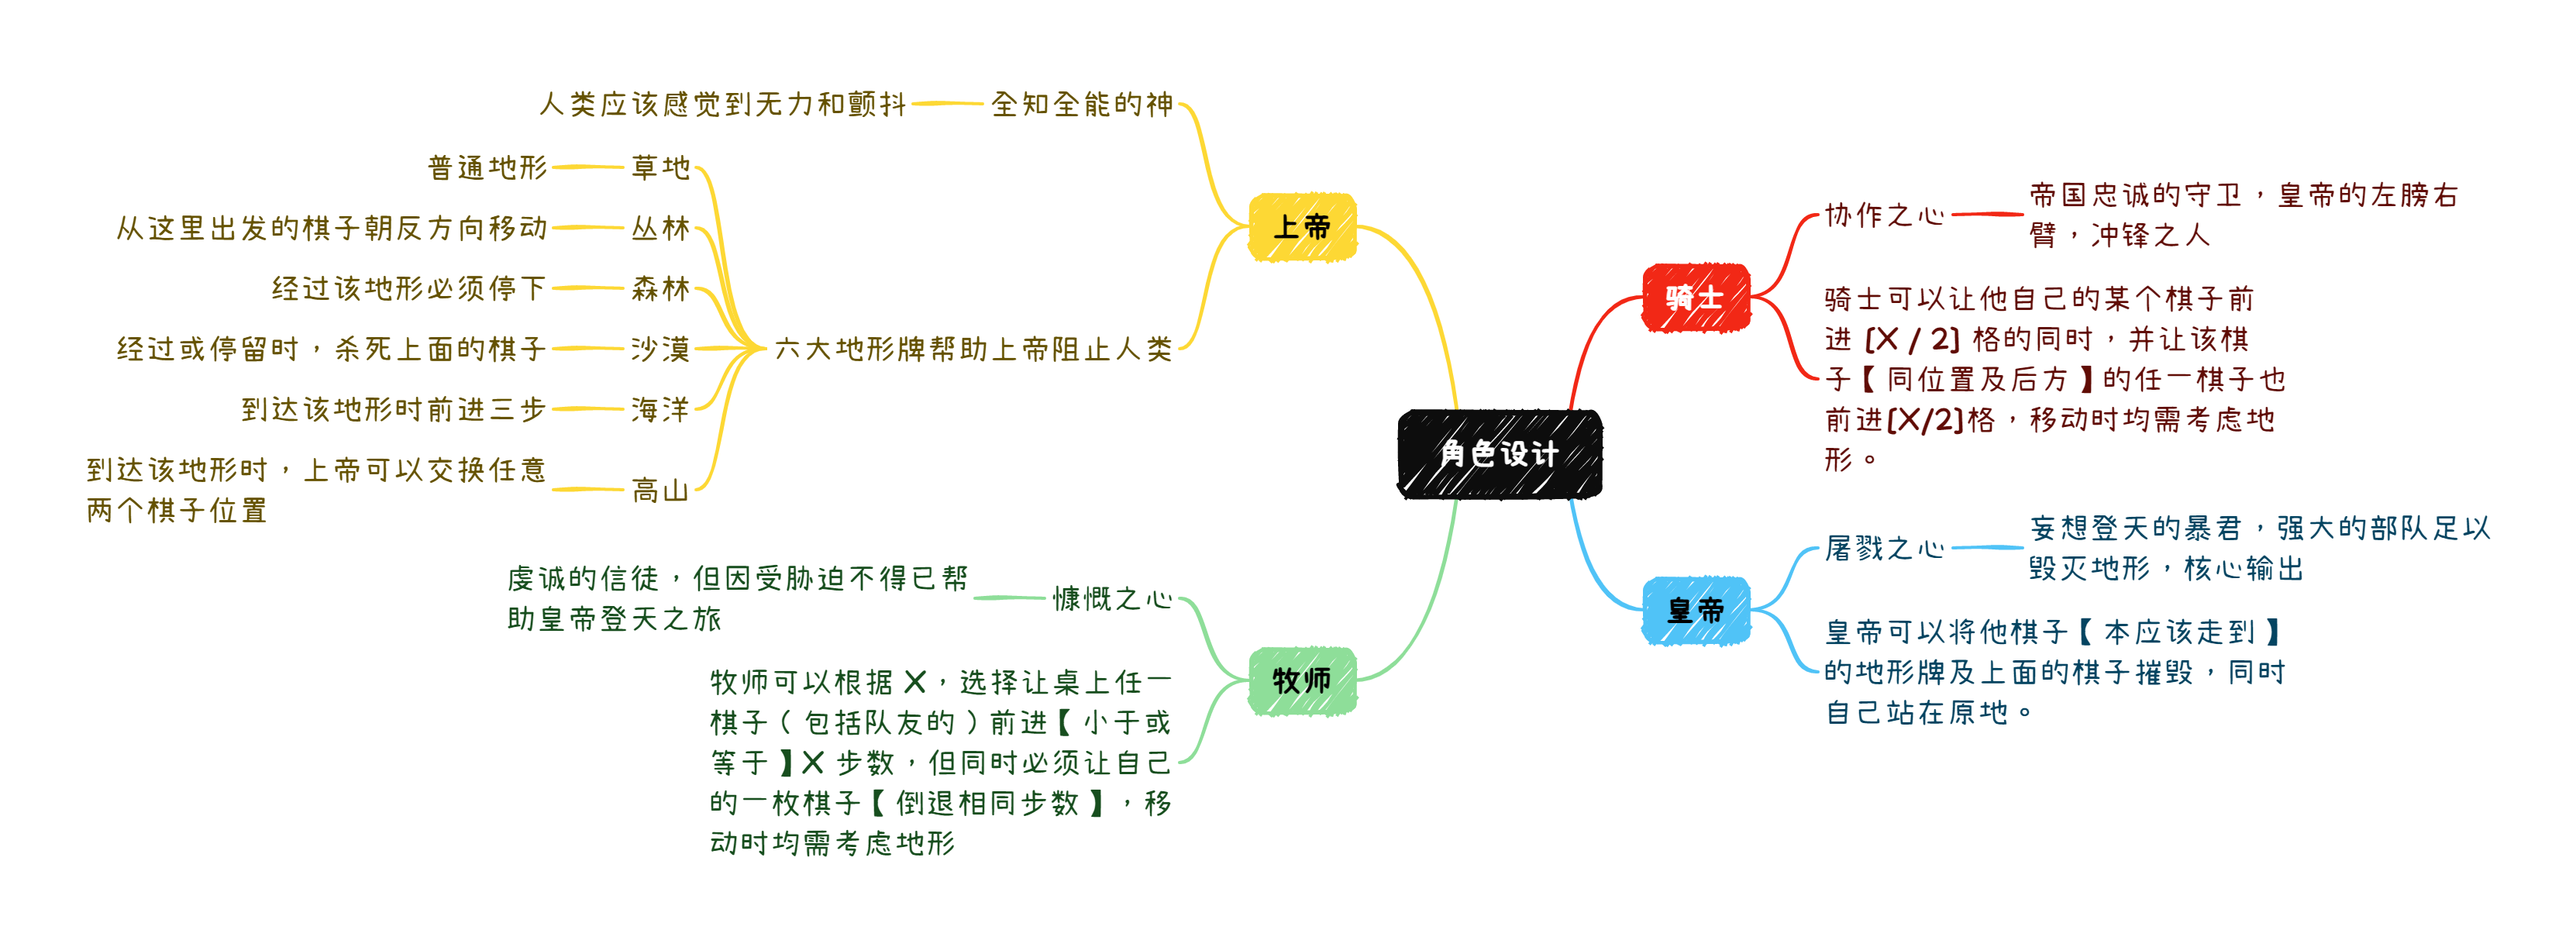
\includegraphics[width=0.9\textwidth]{Images/Up to Heaven/design.png}
    \caption{Up to Heaven\ 角色设计}
    \label{fig:UTH_Design}
\end{figure}

游戏最复杂的地方在于平衡性测试,由于我们体验目标侧重点在于人类登上天堂屠戮上帝,希望人类相互合作、牺牲,最大化自己能力帮助团队,最终艰难地登顶。所以上帝能力如果太弱,无法让玩家感受到登天之难。上帝能力如果太强,人类玩家只会感到无力,所有的策略性选择都是无意义的,“我已经尽力了可我还是输了”。我们进行了一共超过三十轮的迭代,以最终人类四成胜率基本实现体验目标。

\begin{figure}[H]
\centering  %图片全局居中
\subfigure[四大角色]{
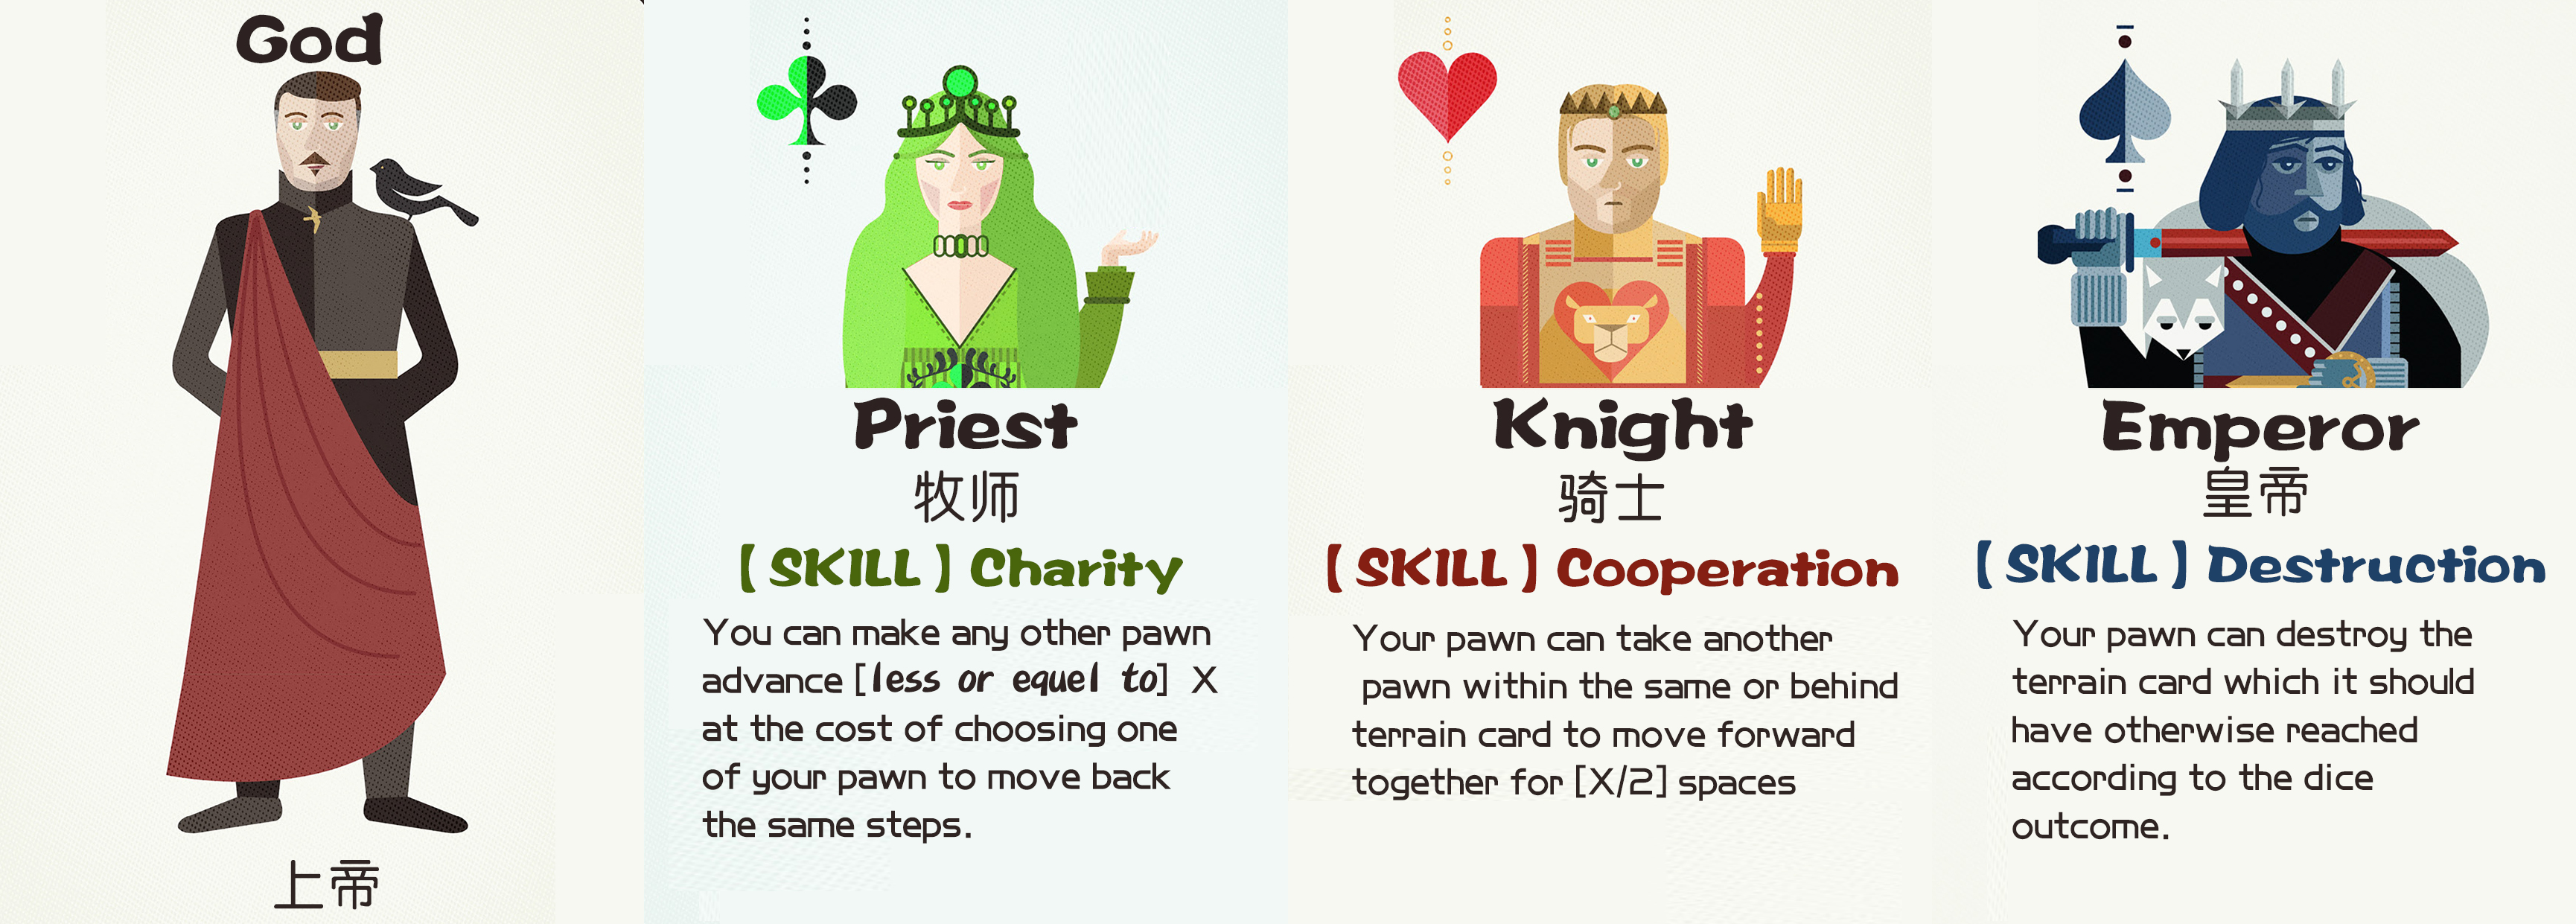
\includegraphics[width=0.45\textwidth]{Images/Up to Heaven/Character.png}}
\subfigure[上帝的地形]{
\includegraphics[width=0.45\textwidth]{Images/Up to Heaven/Up to Heaven.png}}
\caption{游戏呈现}
\end{figure}




\begin{itemize}
    \item \textbf{游戏实况:}  \href{https://www.bilibili.com/video/BV1jL411179M/?vd_source=ead0ac501dfae814e19fd7d9f376d92d}{Bilibili视频}
    \item \textbf{创意工坊:}  \href{https://steamcommunity.com/sharedfiles/filedetails/?id=2847103396}{Steam创意工坊} 
\end{itemize}